\chapter{Описание алгоритмов}

В данной главе будут рассмотрены самые популярные алгоритмы обучения с подкреплением.
Популярность была определена по наличию программной реализации алгоритма в свободном доступе.

\section{Выбор алгоритмов для исследования}

В ходе проведенного анализа репозиториев и библиотек (\cite{samvelyan19smac}, \cite{MARL-ALGORIGHMS}, \cite{Awesome-MARL}) были выделены следующие алгоритмы:

\begin{itemize}[label=---]
	% \item Centralized Q Learning - централизованное Q-обучение;
	\item IQL --- независимое Q--обучение \cite{DBLP:journals/corr/TampuuMKKKAAV15};
	\item VDN --- сети декомпозиции V--функции \cite{DBLP:journals/corr/SunehagLGCZJLSL17};
	\item QMIX --- факторизация монотонной Q--функции \cite{DBLP:journals/corr/abs-1803-11485};
	\item MAVEN ---- несколько агентов с вариационным исследованием \cite{DBLP:journals/corr/abs-1910-07483};
	% \item CommNET ---- обучение коммуникации нескольких агентов используя обратное распространение ошибки \cite{DBLP:journals/corr/SukhbaatarSF16};
	\item MADDPG --- алгоритм DDPG \cite{https://doi.org/10.48550/arxiv.1509.02971} с несколькими агентами \cite{lowe2017multi};
	\item MAPPO --- удивительная эффективность PPO \cite{DBLP:journals/corr/SchulmanWDRK17} в среде с несколькими агентами \cite{DBLP:journals/corr/abs-2103-01955};
	\item IPPO --- обычный алгоритм PPO из обучения с подкреплением в среде с одним агентом.
\end{itemize}

\section{IQL}

Алгоритм строится на основе Deep Q Learning \cite{Mnih2013PlayingAW}, для каждый агент контролируется отдельной сетью.
Агенты играют независимо друг от друга, но видят одну и ту же среду, и действия друг друга.
В качестве среды был выбран модифицированный эмулятор игровой консоли Atari. 
На примере игры в понг протестированы среды, подразумевающие как кооперацию, так и конкуренцию. При кооперации, агенты удерживали мяч на поле наибольшее время.
К недостаткам алгоритма можно отнести отсутствие теоретической гарантии достижения эквилибриума \cite{DBLP:journals/corr/abs-2011-00583}. 

\begin{enumerate}[label={\arabic*)}]
	\item дискретные действия;
	\item алгоритм для смешанных игр;
	\item off--policy;
	\item как во время обучения, так и во время тестирования агенты децентрализованы.
\end{enumerate}

В системе реального мира, где агенты только децентрализованы, такой подход может оказаться единственным возможным.

\section{VDN}

VDN \cite{DBLP:journals/corr/SunehagLGCZJLSL17} пытаются обучить совместную Q--функцию:

\begin{equation}
	Q_{tot} (s, a) = \sum{i \in \mathcal{N}} Q_i(s^i, u^i; \; \theta^i).
\end{equation}

Она отличается от IQL тем, что Q--функциям для каждого агента не поступает информация о состоянии и действиях другого агента.
Таким образом достигается большая автономность агентов. Метод уступает по всем метрикам методу, описанному ниже, и по этой причине не используется в сравнениях. 
Тем не менее, он обладает достаточной методической значимостью, чтобы быть рассмотренным.

Таким образом можно классифицировать алгоритм следующими критериями: 
\begin{enumerate}[label={\arabic*)}]
	\item дискретные действия;
	\item алгоритм для смешанных игр;
	\item off--policy;
	\item во время обучения агенты централизованны, а во время тестирования децентрализованы;
\end{enumerate}

\section{QMIX}

QMIX строится на базе VDN, но вместо суммы используется факторизация монотонной Q--функции по ограничению:

\begin{equation}
	\frac{\partial Q_{tot}}{\partial Q_i} \geq 0,\forall i \in \mathcal{N}.
\end{equation}

Чтобы обеспечить условие выше, QMIX использует 2 дополнительных сети: mixing network, hyper network.
Авторы алгоритма демонстрируют его превосходство над VDN на примере кооперативной игры с суммой матрицы. VQN не удается достичь эквилибриума.

Таким образом можно классифицировать алгоритм следующими критериями:
\begin{enumerate}[label={\arabic*)}]
	\item дискретные действия;
	\item алгоритм для смешанных игр;
	\item off--policy;
	\item во время обучения агенты централизованны, а во время тестирования децентрализованы;
\end{enumerate}

Алгоритм является улучшением VDN.

\section{MAVEN}

Авторы MAVEN замечают, что ограничения, полагаемые QMIX ведут к плохой стратегии исследования среды, как результат к худшей производительности \cite{DBLP:journals/corr/abs-1910-07483}.
MAVEN вводит новый подход совмещающий методы обучения с использованием V-функции и методы с использованием стратегии. Они вводят общее латентное пространство, управляемое иерархической стратегией.

Они предлагают использовать ансамбль генеративных стратегий для управления \(Q_i\), в то же время гарантируя монотонность \(Q_i\) по \(Q_{tot}\).
Таким образом достигается консистентное по времени исследования среды.

\begin{figure}[H]
	\begin{center}
	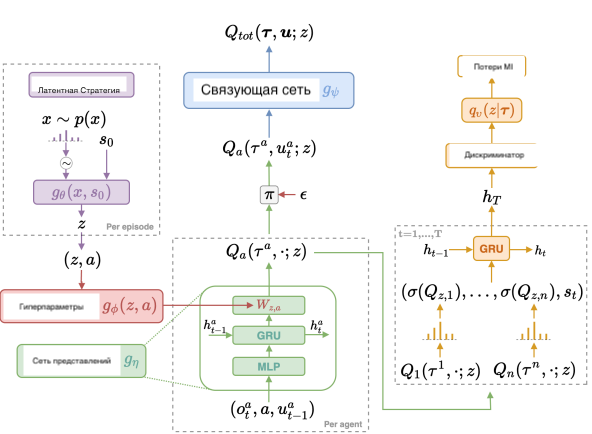
\includegraphics[pages=-, width=140mm]{./inc/img/maven.png}
	\caption{Архитектура MAVEN}
	\label{fig:maven}
\end{center}
\end{figure}

Таким образом можно классифицировать алгоритм следующими критериями:
\begin{enumerate}[label={\arabic*)}]
	\item дискретные действия;
	\item алгоритм для смешанных игр;
	\item off--policy;
	\item во время обучения агенты централизованны, а во время тестирования децентрализованы;
\end{enumerate}

Алгоритм является улучшением QMIX и VDN.

% TODO: Таким образом можно классифицировать алгоритм как 1. алгоритм для смешанных игр, 2. агент наблюдает награду за все действия 3. во время обучения агенты централизованны, а во время тестирования децентрализованы;

% \section{CommNet}
% 
% CommNet предлагает ортогональный подход к MARL. Предыдущие алгоритмы не допускают коммуникации агентов.
% В этом подходе, агенты должны придумать способ общения, чтобы достичь цели. Словами являются континуальные вектора.
% 
% \begin{figure}[H]
% 	\begin{center}
% 	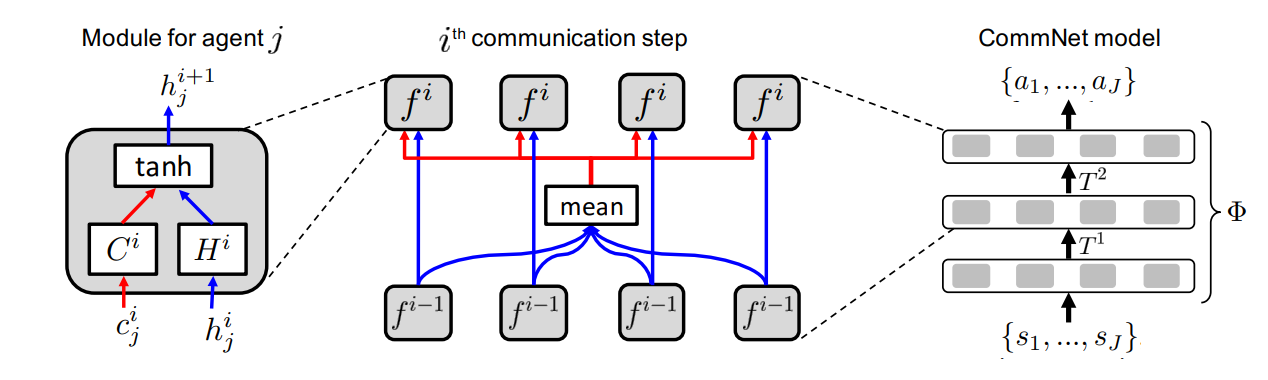
\includegraphics[pages=-, width=140mm]{./inc/img/commnet.png}
% 	\caption{Работа сети CommNet}
% 	\label{fig:commnet}
% \end{center}
% \end{figure}
% 
% Для кодирования состояния используются рекуррентные нейронные сети (\ref{fig:commnet} слева). \( h_j^i \) - скрытое состояние агента \(j\) в момент времени \(i\).
% Нейросеть принимает предыдущее состояние и вектор коммуникации. Вектор коммуникации \(c_j^i\) - это вектор, который агент \(j\) получает от агента \(i\). Вектор коммуникации на следующем шаге - среднее скрытое состояние всех агентов. Вектор коммуникации предоставляется всем агентам на следующем шаге.

\section{Традиционные алгоритмы из обучения с подкреплением}

В данной секции рассказывается про традиционные алгоритмы. 
Среди них PPO, берущий за основу метод Actor-Critic. В контексте нескольких агентов, метод получил название IPPO (независимый PPO) \cite{DBLP:journals/corr/abs-2103-01955}.

Следующие алгоритмы следуют парадигме <<централизованное обучение и децентрализованная игра>> (centralized learning and decentralized execution).
Это классические алгоритмы DDPG и PPO, оснащенные центральной Q-сетью. Они названы MADDPG и MAPPO соответственно \cite{https://doi.org/10.48550/arxiv.1509.02971}.
В сравнениях ниже также представлен MAA2C, который является адаптацией A2C для нескольких агентов. IA2C - это независимая версия A2C.

Классификация IPPO может быть сделана по следующим критериям:
\begin{enumerate}[label={\arabic*)}]
	\item смешанные действия;
	\item алгоритм для смешанных игр;
	\item on--policy;
	\item полная децентрализация;
\end{enumerate}

Метод IPPO подходит для сценариев, когда не хранится буфер наблюдений среды, а агенты обучаются по мере игры.
Также стоит отметить его простоту реализации, и факт полной децентрализации.

Классификация других методов может быть сделана по следующим критериям:
\begin{enumerate}[label={\arabic*)}]
	\item смешанные действия;
	\item алгоритм для смешанных игр;
	\item централизованное обучение и децентрализованная тестирование;
\end{enumerate}

\subsection*{Вывод}

Был проведен анализ релевантности алгоритмов, выделены популярные алгоритмы для анализа в данной работе, приведено их краткое описание, основные свойства, классификация.